%%%%%%%%%%%%%%%%%%%%%%%%%%%%%%%%%%%%%%%%%
% Beamer Presentation
% LaTeX Template
% Version 1.0 (10/11/12)
%
% This template has been downloaded from:
% http://www.LaTeXTemplates.com
%
% License:
% CC BY-NC-SA 3.0 (http://creativecommons.org/licenses/by-nc-sa/3.0/)
%
%%%%%%%%%%%%%%%%%%%%%%%%%%%%%%%%%%%%%%%%%

%----------------------------------------------------------------------------------------
%	PACKAGES AND THEMES
%----------------------------------------------------------------------------------------

%\documentclass[UTF8,aspectratio=169,14pt]{ctexbeamer}
\documentclass[UTF8,aspectratio=169]{ctexbeamer}
\usepackage{hyperref}
\hypersetup{
	colorlinks=true,
	linkcolor=red,
	anchorcolor=blue,
	citecolor=green
}

\mode<presentation> {
	
	% The Beamer class comes with a number of default slide themes
	% which change the colors and layouts of slides. Below this is a list
	% of all the themes, uncomment each in turn to see what they look like.
	
	%\usetheme{default}
	%\usetheme{AnnArbor}
	%\usetheme{Antibes}
	%\usetheme{Bergen}
	%\usetheme{Berkeley}
	%\usetheme{Berlin}
	%\usetheme{Boadilla}
	%\usetheme{CambridgeUS}
	%\usetheme{Copenhagen}
	%\usetheme{Darmstadt}
	%\usetheme{Dresden}
	%\usetheme{Frankfurt}
	%\usetheme{Goettingen}
	%\usetheme{Hannover}
	%\usetheme{Ilmenau}
	%\usetheme{JuanLesPins}
	%\usetheme{Luebeck}
	\usetheme{Madrid}
	%\usetheme{Malmoe}
	%\usetheme{Marburg}
	%\usetheme{Montpellier}
	%\usetheme{PaloAlto}
	%\usetheme{Pittsburgh}
	%\usetheme{Rochester}
	%\usetheme{Singapore}
	%\usetheme{Szeged}
	%\usetheme{Warsaw}
	
	% As well as themes, the Beamer class has a number of color themes
	% for any slide theme. Uncomment each of these in turn to see how it
	% changes the colors of your current slide theme.
	
	%\usecolortheme{albatross}
	%\usecolortheme{beaver}
	%\usecolortheme{beetle}
	%\usecolortheme{crane}
	%\usecolortheme{dolphin}
	%\usecolortheme{dove}
	%\usecolortheme{fly}
	%\usecolortheme{lily}
	%\usecolortheme{orchid}
	%\usecolortheme{rose}
	%\usecolortheme{seagull}
	%\usecolortheme{seahorse}
	%\usecolortheme{whale}
	%\usecolortheme{wolverine}
	
	%\setbeamertemplate{footline} % To remove the footer line in all slides uncomment this line
	%\setbeamertemplate{footline}[page number] % To replace the footer line in all slides with a simple slide count uncomment this line
	
	%\setbeamertemplate{navigation symbols}{} % To remove the navigation symbols from the bottom of all slides uncomment this line
}

\usepackage{graphicx} % Allows including images
\graphicspath{{./figs/}}
\usepackage{booktabs} % Allows the use of \toprule, \midrule and \bottomrule in tables
\usepackage{longtable}
\usepackage{listings}
\usepackage{xcolor}
\lstset{numbers=left, %设置行号位置
	numberstyle=\tiny, %设置行号大小
	keywordstyle=\color{blue}, %设置关键字颜色
	commentstyle=\color[cmyk]{1,0,1,0}, %设置注释颜色
	frame=single, %设置边框格式
	escapeinside=``, %逃逸字符(1左面的键),用于显示中文
	%breaklines, %自动折行
	extendedchars=false, %解决代码跨页时,章节标题,页眉等汉字不显示的问题
	xleftmargin=2em,xrightmargin=2em, aboveskip=1em, %设置边距
	tabsize=4, %设置tab空格数
	showspaces=false %不显示空格
}
% Fonts
% \usepackage{libertine}
% \setmonofont{Courier}
\setCJKsansfont[ItalicFont=Noto Serif CJK SC Black, BoldFont=Noto Sans CJK SC Black]{Noto Sans CJK SC}
\setmainfont[Ligatures={Common,TeX}]{Linux  Libertine O}
\setmonofont[SmallCapsFont={Latin Modern Mono Caps}]{Latin Modern Mono Light}
\setsansfont{Linux Biolinum O}

\logo{
\includegraphics[width=0.55cm,height=0.55cm]{../../thcs-logo.png}}

%----------------------------------------------------------------------------------------
%	TITLE PAGE
%----------------------------------------------------------------------------------------

\title[第7讲]{第7讲 :Scalable Synchronization on Shared-Memory Multiprocessors} % The short title appears at the bottom of every slide, the full title is only on the title page
\subtitle{第二节:Hardware Behavior in Shared-Memory Multiprocessors -- Cache Coherence}
\author{陈渝} % Your name
\institute[清华大学] % Your institution as it will appear on the bottom of every slide, may be shorthand to save space
{
	清华大学计算机系 \\ % Your institution for the title page
	\medskip
	\textit{yuchen@tsinghua.edu.cn} % Your email address
}
\date{\today} % Date, can be changed to a custom date


\begin{document}

\begin{frame}
\titlepage % Print the title page as the first slide
\end{frame}

%\begin{frame}
%\frametitle{提纲} % Table of contents slide, comment this block out to remove it
%\tableofcontents % Throughout your presentation, if you choose to use \section{} and \subsection{} commands, these will automatically be printed on this slide as an overview of your presentation
%\end{frame}
%
%%----------------------------------------------------------------------------------------
%%	PRESENTATION SLIDES
%%----------------------------------------------------------------------------------------
%
%%------------------------------------------------
%\section{第一节:课程概述} % Sections can be created in order to organize your presentation into discrete blocks, all sections and subsections are automatically printed in the table of contents as an overview of the talk
%%------------------------------------------------
%-------------------------------------------------
\begin{frame}[plain]
	\frametitle{Introduction -- Baseline system model}


			\centering
			
			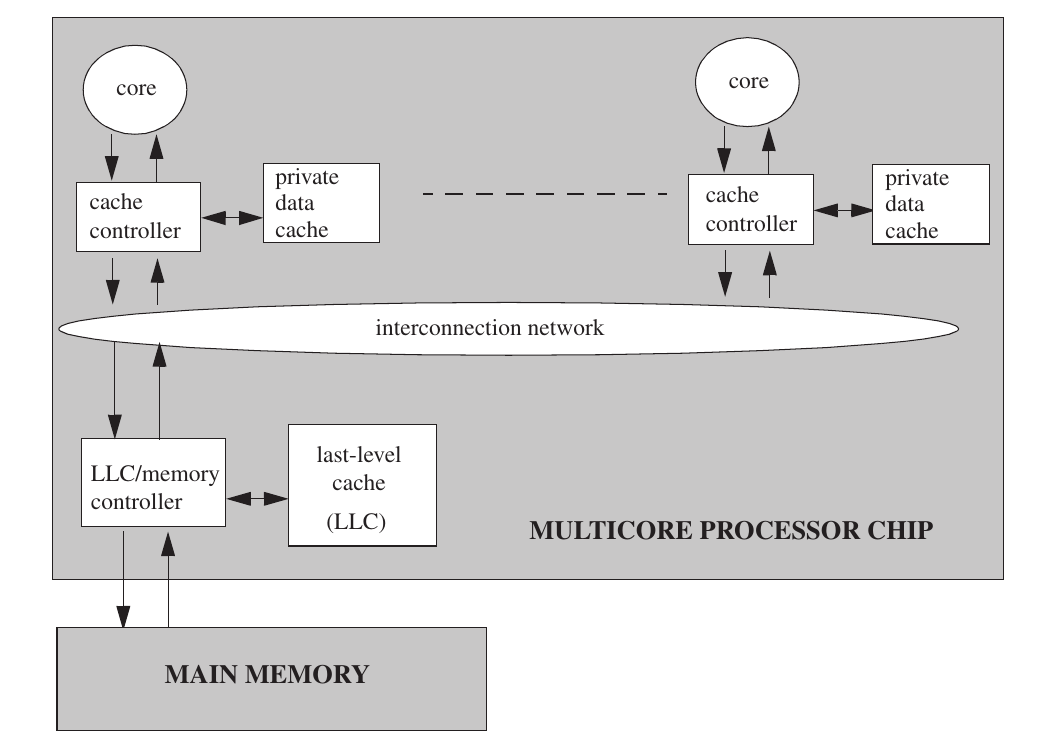
\includegraphics[width=.6\textwidth]{baseline-system}


%左对齐、居中对齐、右对齐的环境分别为flushleft、center和flushright。也可以使用命令\raggedright、\centering和\raggedleft使以后的文本按指定方式对齐.
\raggedright
\tiny ref:
Some info are from

Paul McKenney (IBM) Tom Hart (University of Toronto), Frans Kaashoek (MIT), 
Daniel J. Sorin "A Primer on Memory Consistency and Cache Coherence",  Fabian Giesen "Cache coherency primer", Mingyu Gao(Tsinghua),Yubin Xia(SJTU)	
\end{frame}

%----------------------------------------------
\begin{frame}[plain]	
	\frametitle{Introduction}
	
	
	\begin{columns}
		
		\begin{column}{.4\textwidth}
			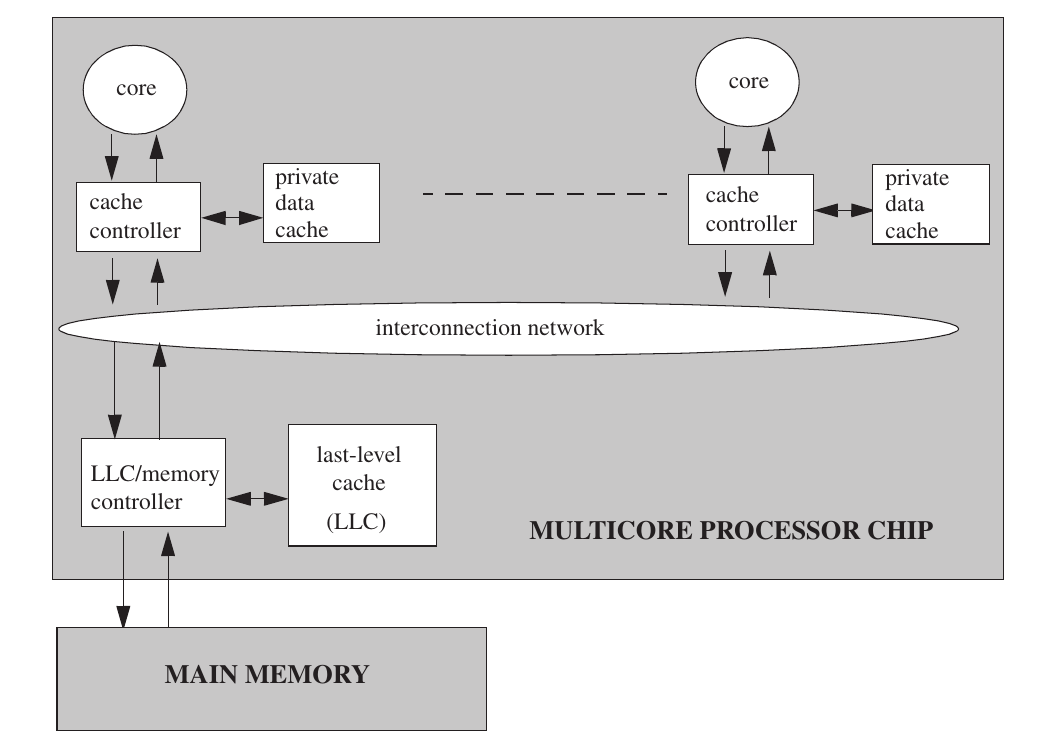
\includegraphics[width=1.\textwidth]{baseline-system}
		\end{column}
		\begin{column}{.6\textwidth}
%			\Large \centering
			基本知识回顾 --缓存(Cache)
			\begin{itemize}
				\item 在现代的CPU上,基本上所有的内存访问都需要通过多层次的缓存来进行。
				\item 例外:比如,对映射成内存地址的 I/O 口,这些访问至少会绕开这个流程的一部分。
				\item CPU 的读 / 写(以及取指令)单元正常情况下甚至都不能直接访问内存——这是物理结构决定的。
				\item 缓存是分“段”(line)的,一个段对应一块存储空间,大小是 32、64、128字节。
			\end{itemize}

		\end{column}
	\end{columns}
	
\end{frame}

%-------------------------------------------------
\begin{frame}[plain]
	\frametitle{Introduction -- Example of incoherence}
   如果有多个核,每个核又都有自己的缓存,那么我们就遇到问题了:如果某个 CPU 缓存段中对应的内存内容被另外一个 CPU 偷偷改了,会发生什么?
	
	Example of incoherence. 
	
%	\centering
	
	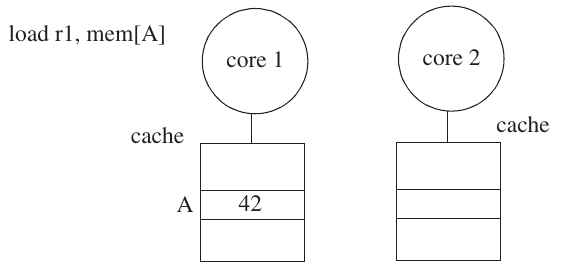
\includegraphics[width=.4\textwidth]{incoherence-ex1}
	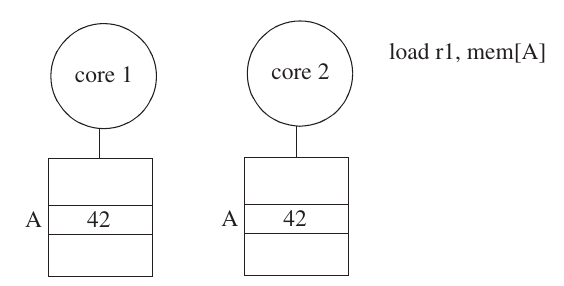
\includegraphics[width=.4\textwidth]{incoherence-ex2}
	\centering
	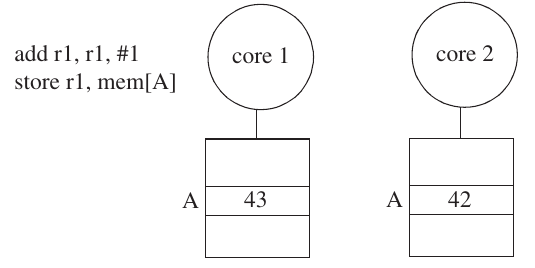
\includegraphics[width=.4\textwidth]{incoherence-ex3}
\end{frame}


%-------------------------------------------------
\begin{frame}[plain]
	\frametitle{Introduction -- define of coherence}
	The basis of our preferred definition of coherence is the single-writer–multiple-reader (SWMR)
	invariant. 
	
	\begin{block}{Coherence invariants}
	1. \textbf{Single-Writer, Multiple-Read (SWMR) Invariant.} For any memory location A, at any
	given (logical) time, there exists only a single core that may write to A (and can also read it)
	or some number of cores that may only read A.
	
	2.  \textbf{Data-Value Invariant.} The value of the memory location at the start of an epoch is the same
	as the value of the memory location at the end of its last read–write epoch.
	
\end{block}
\pause
如果一个 CPU 缓存了某块内存,那么在其他 CPU 修改这块内存的时候,我们希望得到通知。我们拥有多组缓存的时候,真的需要它们保持同步。

或者说,系统的内存在各个 CPU 之间无法做到与生俱来的同步,我们实际上是需要一个大家都能遵守的方法来达到同步的目的。

\end{frame}


%-------------------------------------------------
\begin{frame}[plain]
	\frametitle{Introduction -- define of coherence}
	
	A shared-memory system is coherent if the results of a parallel program
	execution are such that:
	\begin{block}{Define of Coherence}

		
		For each memory location, the result is the same as the result of a
		hypothetical serialization of all memory accesses by all cores to the
		location, and in the serialization:
		
		1. Memory accesses by any one core keeps the order
		
		
		2. Each load returns the value written by the last write
		
		
	\end{block}
	

	
\end{frame}



%----------------------------------------------
\begin{frame}[plain]	
	\frametitle{Introduction -- 一致性协议(Coherency protocols) }
	
	
	\begin{columns}
		
		\begin{column}{.4\textwidth}
			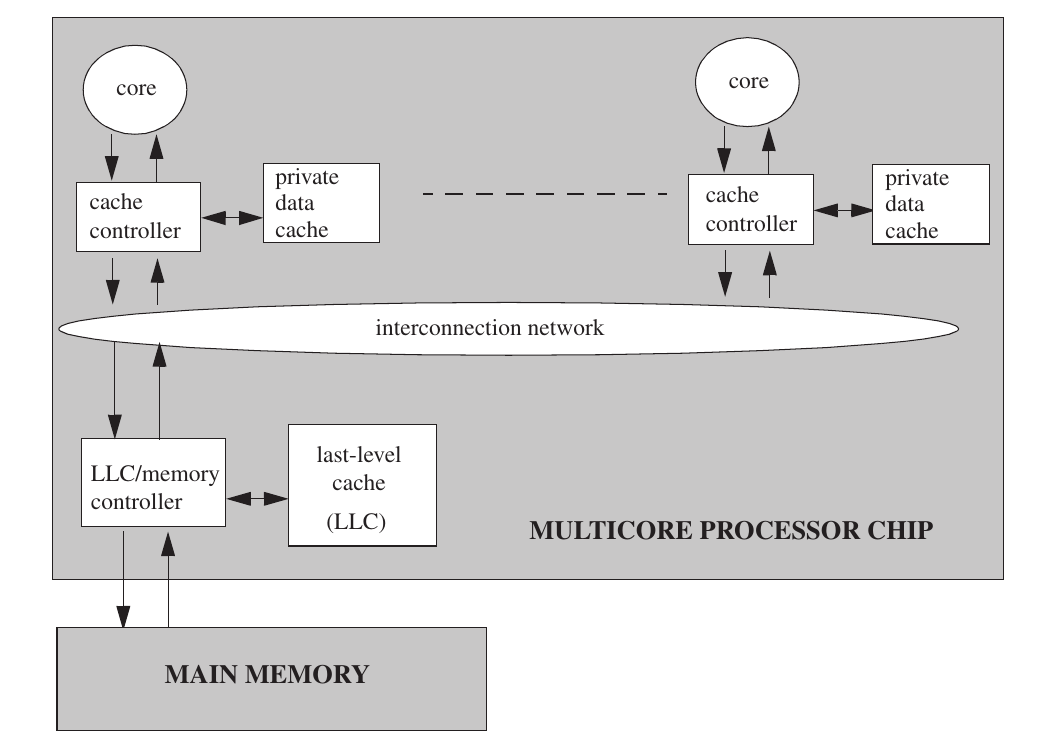
\includegraphics[width=1.\textwidth]{baseline-system}
		\end{column}
		\begin{column}{.6\textwidth}
			%			\Large \centering
			解决问题的方法 1: 共用一组缓存
			\begin{itemize}
				\item 这个问题的根源是我们拥有多组缓存,而不是多个 CPU 核
				\item 让多个 CPU 核共用一组缓存
				\item 在每一个指令周期,只有一个幸运的 CPU 能通过一级缓存做内存操作,运行它的指令
			\end{itemize}
			问题 
			\pause
			: 太慢!
		\end{column}
	\end{columns}
	
\end{frame}


%----------------------------------------------
\begin{frame}[plain]	
	\frametitle{Introduction -- MSI一致性协议}
	
	
	\begin{columns}
		
		\begin{column}{.4\textwidth}
			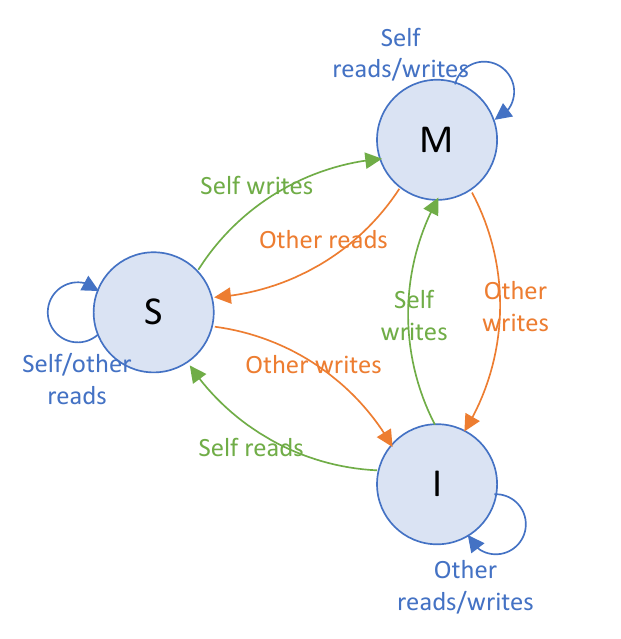
\includegraphics[width=1.\textwidth]{msi-states}
		\end{column}
		\begin{column}{.6\textwidth}
			%			\Large \centering
			解决问题的方法 2: MSI一致性协议
			
			MSI 是三种缓存段状态的首字母缩写,任何多核系统中的缓存段都处于这三种状态之一。
			\begin{itemize}
				\item M(odified):One cache (single writer) has valid and latest copy, and can write. Memory copy is stale.
				\item S(hared): One or more caches (multiple readers) and memory have valid copy.
				\item I(nvalid): Not present.
			\end{itemize}
			
		\end{column}
	\end{columns}
	
\end{frame}



%----------------------------------------------
\begin{frame}[plain]	
	\frametitle{Introduction -- MSI一致性协议}
	
	
	\begin{columns}
		
		\begin{column}{.4\textwidth}
			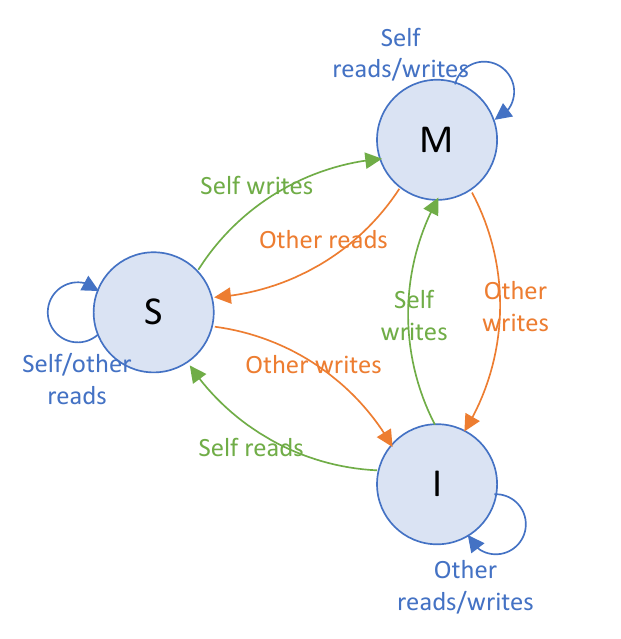
\includegraphics[width=1.\textwidth]{msi-states}
		\end{column}
		\begin{column}{.6\textwidth}
			%			\Large \centering
			解决问题的方法 2: MSI一致性协议
			
			Self read/write triggers up transition
			\begin{itemize}
				\item  I -> S				
				\item  S -> M (upgrade)				
			\end{itemize}
			Other read/write triggers down transition
			\begin{itemize}
				\item  M -> S (downgrade)			
				\item  S -> I (invalidate)				
			\end{itemize}			
			Obtains exclusive ownership before write
			\begin{itemize}
				\item  Needs to upgrade even if hit in S			
				\item Causes others to invalidate
				\item If M in another cache, will cause writeback

			\end{itemize}					
		\end{column}
	\end{columns}
	
\end{frame}

%----------------------------------------------
\begin{frame}[plain]	
    \frametitle{Introduction -- MESI一致性协议}
    
    
    \begin{columns}
        
        \begin{column}{.4\textwidth}
            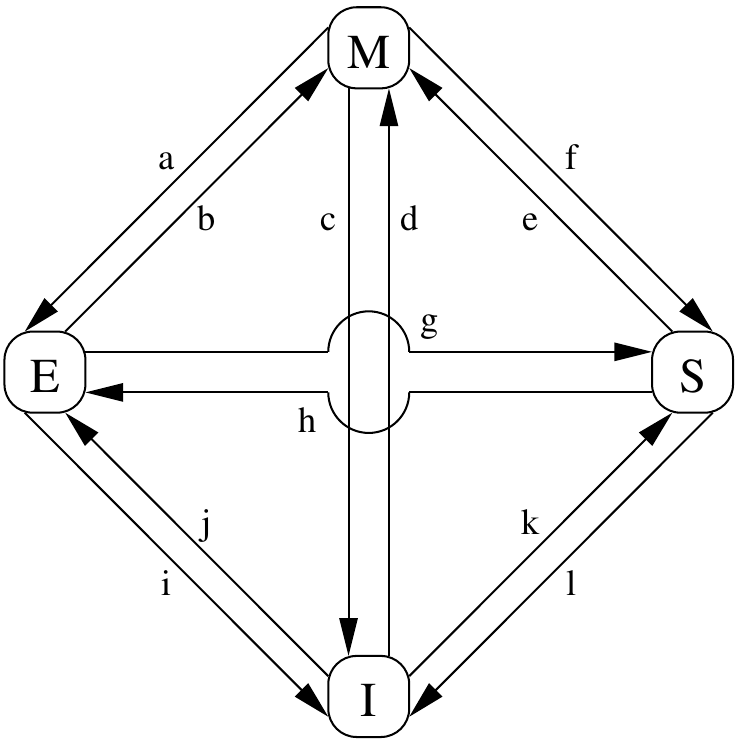
\includegraphics[width=1.\textwidth]{mesi-state}
        \end{column}
        \begin{column}{.6\textwidth}
            %			\Large \centering
            解决问题的方法 3: MESI一致性协议
            
            Protocol Optimization – E State
            
            Scenario: private data to a core is first read and then later written
            
            With MSI protocol: two broadcast bus transactions
            \begin{itemize}				
                \item One BRd for I -> S :  CRd/BRd
                \item  One BRdX for S -> M : CWr/BRdX
            \end{itemize}
            
            With MESI protocol: one bus transaction
            \begin{itemize}	
                \item First I -> E  : CRd/BRd
                \item E -> M  : silently upgrade, no bus transaction since we know it is the only copy
                \item E -> S: downgrade if sharing				
            \end{itemize}		
            
        \end{column}
    \end{columns}
    
\end{frame}
%----------------------------------------------
\begin{frame}[plain]	
	\frametitle{Introduction -- MESI一致性协议}
	
	
	\begin{columns}
		
		\begin{column}{.4\textwidth}
			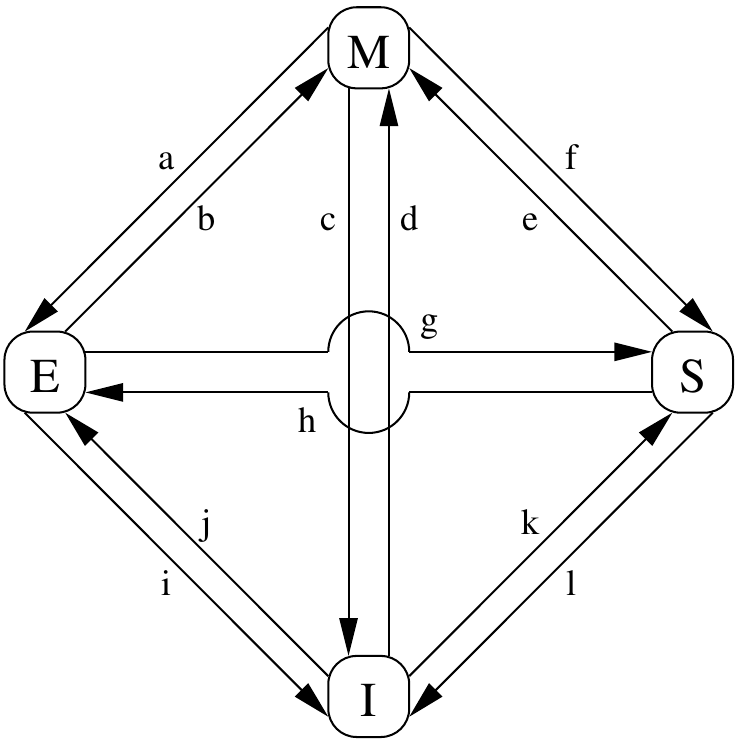
\includegraphics[width=1.\textwidth]{mesi-state}
		\end{column}
		\begin{column}{.6\textwidth}
			%			\Large \centering
			解决问题的方法 3: MESI一致性协议
			
			MESI 是四种缓存段状态的首字母缩写,任何多核系统中的缓存段都处于这四种状态之一。
			\begin{itemize}
				\item 失效(Invalid)缓存段,要么已经不在缓存中,要么它的内容已经过时。为了达到缓存的目的,这种状态的段将会被忽略。一旦缓存段被标记为失效,那效果就等同于它从来没被加载到缓存中。
				\item 共享(Shared)缓存段,它是和主内存内容保持一致的一份拷贝,在这种状态下的缓存段只能被读取,不能被写入。多组缓存可以同时拥有针对同一内存地址的共享缓存段,这就是名称的由来。
%				\item 独占(Exclusive)缓存段,和 S 状态一样,也是和主内存内容保持一致的一份拷贝。区别在于,如果一个处理器持有了某个 E 状态的缓存段,那其他处理器就不能同时持有它,所以叫“独占”。这意味着,如果其他处理器原本也持有同一缓存段,那么它会马上变成“失效”状态。
%				\item 已修改(Modified)缓存段,属于脏段,它们已经被所属的处理器修改了。如果一个段处于已修改状态,那么它在其他处理器缓存中的拷贝马上会变成失效状态,这个规律和 E 状态一样。此外,已修改缓存段如果被丢弃或标记为失效,那么先要把它的内容回写到内存中——这和回写模式下常规的脏段处理方式一样。
			\end{itemize}
]
		\end{column}
	\end{columns}
	
\end{frame}


%----------------------------------------------
\begin{frame}[plain]	
	\frametitle{Introduction -- MESI一致性协议}
	
	
	\begin{columns}
		
		\begin{column}{.4\textwidth}
			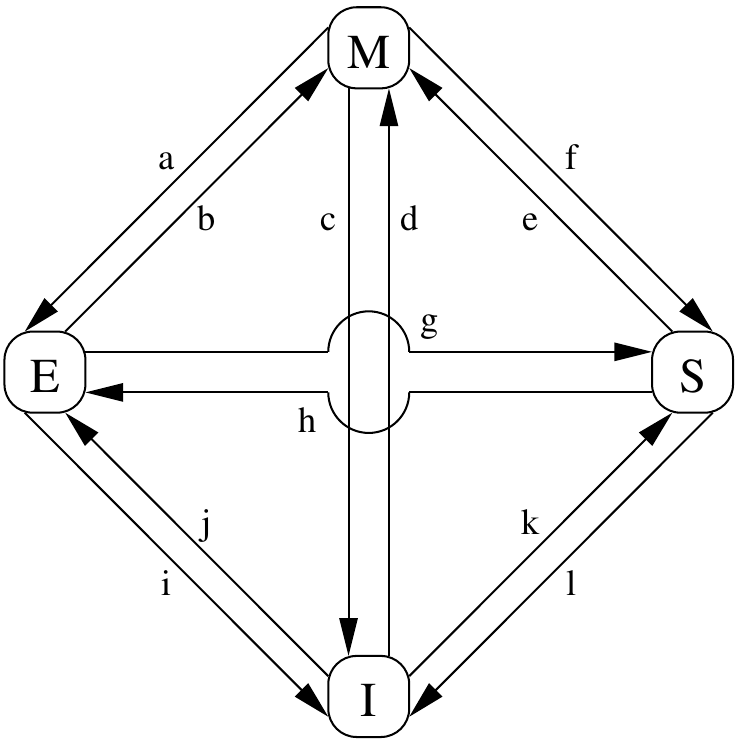
\includegraphics[width=1.\textwidth]{mesi-state}
		\end{column}
		\begin{column}{.6\textwidth}
			%			\Large \centering
			解决问题的方法 3: MESI一致性协议
			
			MESI 是四种缓存段状态的首字母缩写,任何多核系统中的缓存段都处于这四种状态之一。
			\begin{itemize}
%				\item 失效(Invalid)缓存段,要么已经不在缓存中,要么它的内容已经过时。为了达到缓存的目的,这种状态的段将会被忽略。一旦缓存段被标记为失效,那效果就等同于它从来没被加载到缓存中。
%				\item 共享(Shared)缓存段,它是和主内存内容保持一致的一份拷贝,在这种状态下的缓存段只能被读取,不能被写入。多组缓存可以同时拥有针对同一内存地址的共享缓存段,这就是名称的由来。

				\item 已修改(Modified)缓存段,属于脏段,它们已经被所属的处理器修改了。如果一个段处于已修改状态,那么它在其他处理器缓存中的拷贝马上会变成失效状态,这个规律和 E 状态一样。此外,已修改缓存段如果被丢弃或标记为失效,那么先要把它的内容回写到内存中——这和回写模式下常规的脏段处理方式一样。
				\item 独占(Exclusive)缓存段,和 S 状态一样,也是和主内存内容保持一致的一份拷贝。区别在于,如果一个处理器持有了某个 E 状态的缓存段,那其他处理器就不能同时持有它,所以叫“独占”。这意味着,如果其他处理器原本也持有同一缓存段,那么它会马上变成“失效”状态。
			\end{itemize}

		\end{column}
	\end{columns}
	
\end{frame}





%----------------------------------------------
\begin{frame}[plain]	
	\frametitle{Introduction -- MESI一致性协议}
	
	
	\begin{columns}
		
		\begin{column}{.4\textwidth}
			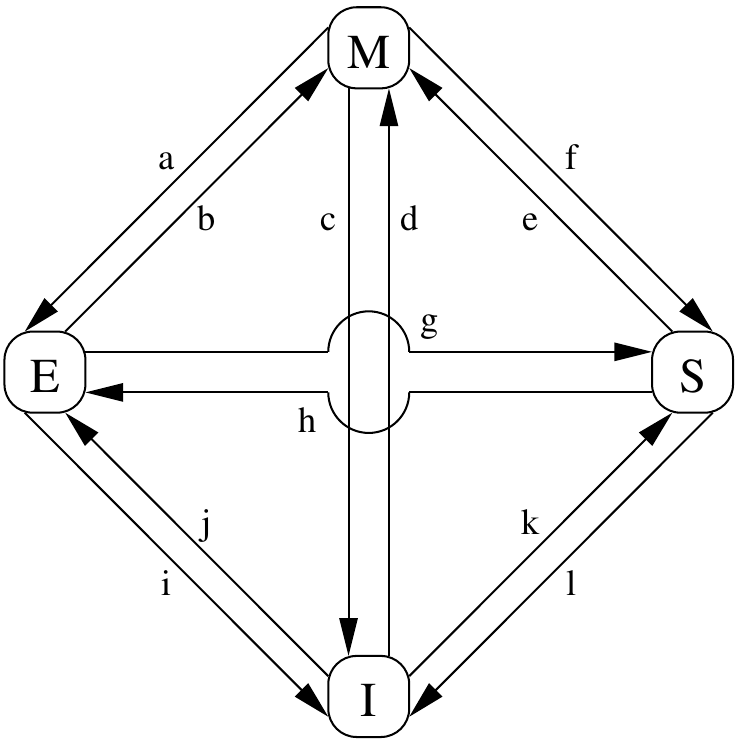
\includegraphics[width=1.\textwidth]{mesi-state}
		\end{column}
		\begin{column}{.6\textwidth}
			%			\Large \centering
			解决问题的方法 3: MESI一致性协议
			
			MESI 是四种缓存段状态的首字母缩写,任何多核系统中的缓存段都处于这四种状态之一。
			\begin{itemize}
				\item 如果把以上这些状态和单核系统中回写模式的缓存做对比,你会发现 I、S 和 M 状态已经有对应的概念:失效 / 未载入、干净以及脏的缓存段。
			\end{itemize}
			
		\end{column}
	\end{columns}
	
\end{frame}


%----------------------------------------------
\begin{frame}[plain]	
	\frametitle{Introduction -- MESI一致性协议}
	
	
	\begin{columns}
		
		\begin{column}{.4\textwidth}
			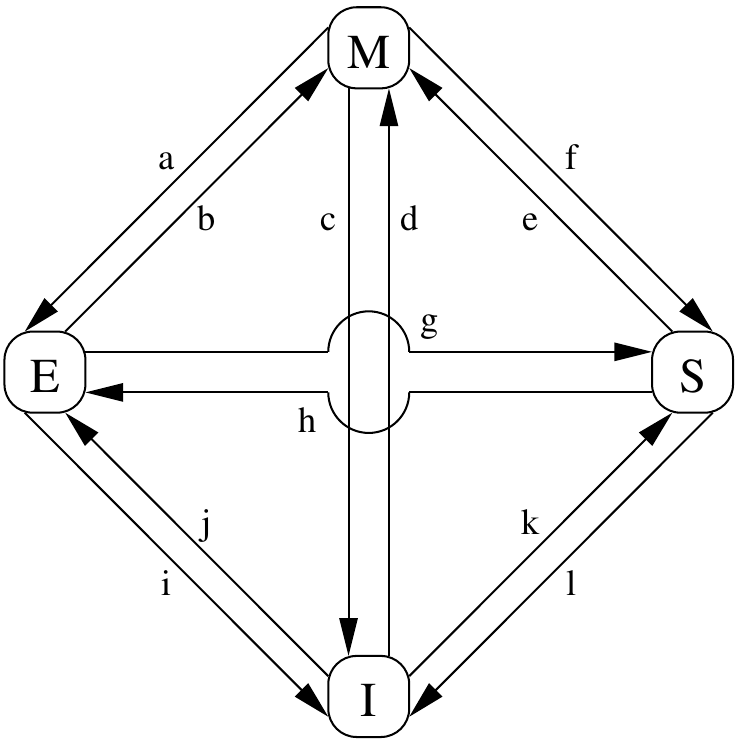
\includegraphics[width=1.\textwidth]{mesi-state}
		\end{column}
		\begin{column}{.6\textwidth}
			%			\Large \centering
			解决问题的方法 3: MESI一致性协议
			
			MESI 是四种缓存段状态的首字母缩写,任何多核系统中的缓存段都处于这四种状态之一。
			\begin{itemize}

				\item 这里的新知识只有 E 状态,代表独占式访问。这个状态解决了“在我们开始修改某块内存之前,我们需要告诉其他处理器”这一问题:只有当缓存段处于 E 或 M 状态时,处理器才能去写它,也就是说只有这两种状态下,处理器是独占这个缓存段的。
			\end{itemize}
			
		\end{column}
	\end{columns}
	
\end{frame}


%----------------------------------------------
\begin{frame}[plain]	
	\frametitle{Introduction -- MESI一致性协议}
	
	
	\begin{columns}
		
		\begin{column}{.4\textwidth}
			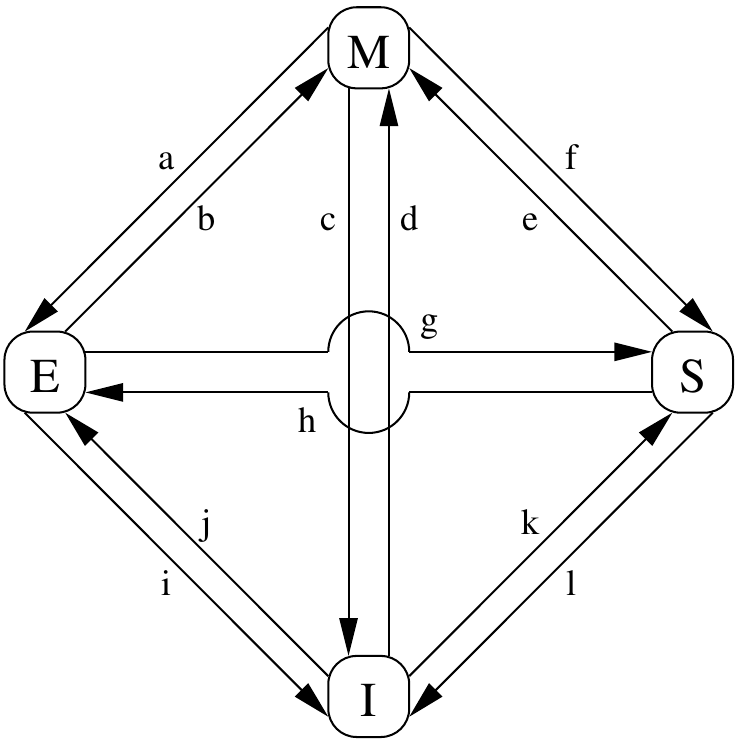
\includegraphics[width=1.\textwidth]{mesi-state}
		\end{column}
		\begin{column}{.6\textwidth}
			%			\Large \centering
			解决问题的方法 3: MESI一致性协议
			
			MESI 是四种缓存段状态的首字母缩写,任何多核系统中的缓存段都处于这四种状态之一。
			\begin{itemize}
				
				\item 当处理器想写某个缓存段时,如果它没有独占权,它必须先发送一条“我要独占权”的请求给总线,这会通知其他处理器,把它们拥有的同一缓存段的拷贝失效(如果它们有的话)。只有在获得独占权后,处理器才能开始修改数据——并且此时,这个处理器知道,这个缓存段只有一份拷贝,在我自己的缓存里,所以不会有任何冲突。
			\end{itemize}
			
		\end{column}
	\end{columns}
	
\end{frame}

%----------------------------------------------
\begin{frame}[plain]	
    \frametitle{Introduction -- MESI一致性协议}
    
    
    \begin{columns}
        
        \begin{column}{.4\textwidth}
            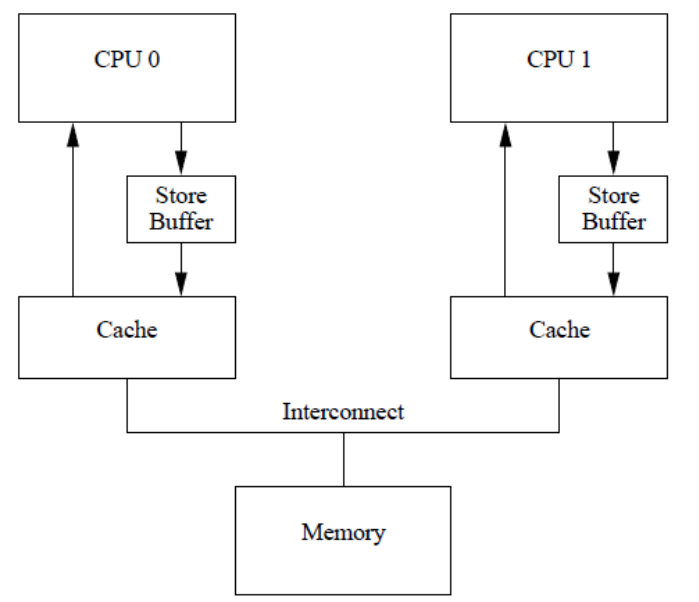
\includegraphics[width=1.\textwidth]{mesi-storebuffer}
        \end{column}
        \begin{column}{.6\textwidth}
            %			\Large \centering
            解决问题的方法 3: MESI一致性协议
            
            MESI 解决了 cache 数据一致性的问题,但
            cpu core之间通信存在延迟,所以在 cpu core 与 cache 中
            间加入了 store buffers。
            
            加入了 store buffers,解决了 Stalls的性能问题, 但是又引入了新的问题:
            store buffers 与 cache 数据的不一致性问题。
            
        \end{column}
    \end{columns}
    
\end{frame}

%----------------------------------------------
\begin{frame}[plain]	
    \frametitle{Introduction -- MESI一致性协议}
    
    
    \begin{columns}
        
        \begin{column}{.4\textwidth}
            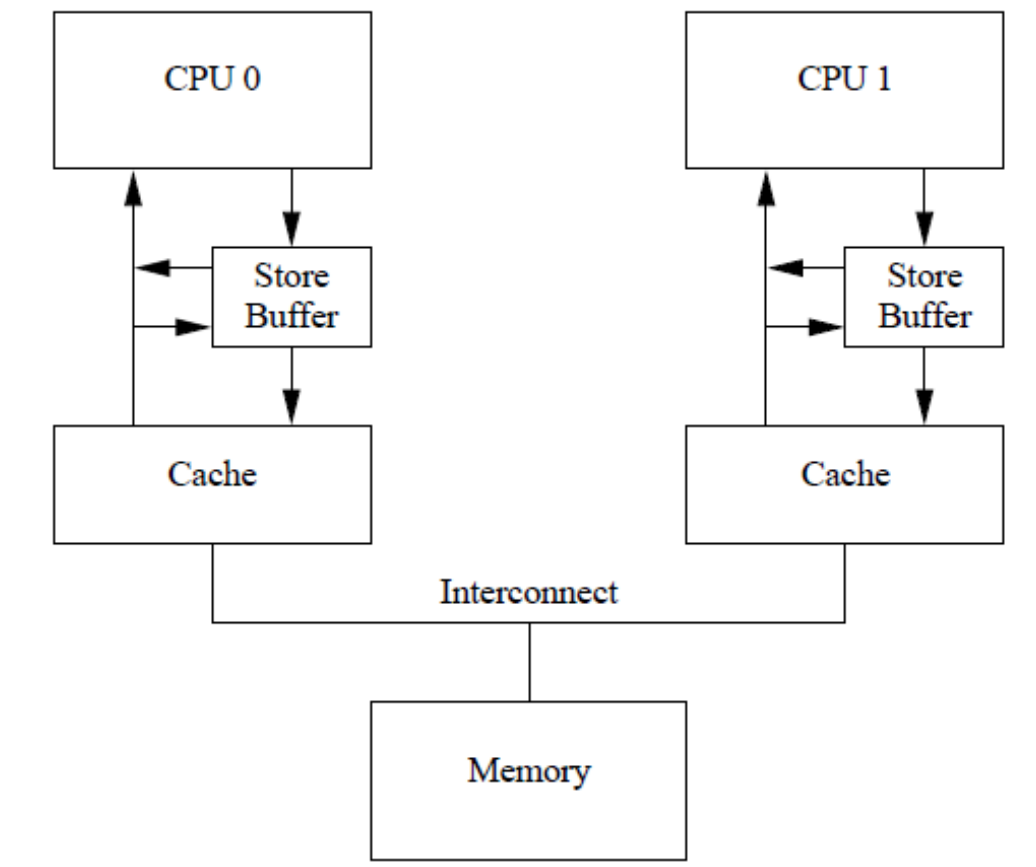
\includegraphics[width=1.\textwidth]{mesi-sb-direct}
        \end{column}
        \begin{column}{.6\textwidth}
            %			\Large \centering
            解决问题的方法 3: MESI一致性协议
       
            Store Buffer
            
            ===========
                        
            加入了 store buffers,解决了 Stalls的性能问题, 但是又引入了新的问题:
            store buffers 与 cache 数据的不一致性问题。
            
            从硬件角度来看,需要引入了
            Store Forwarding机制:即可以通过store buffer把一个特定 CPU 的 store 直接转给它
            随后的加载,而不通过 cache。这样避免了 cpu 取 cache 数据与
            store buffer 数据的不一致问题。
            
            
            
        \end{column}
    \end{columns}
    
\end{frame}

%----------------------------------------------
\begin{frame}[plain]	
    \frametitle{Introduction -- MESI一致性协议}
    
    
    \begin{columns}
        
        \begin{column}{.4\textwidth}
            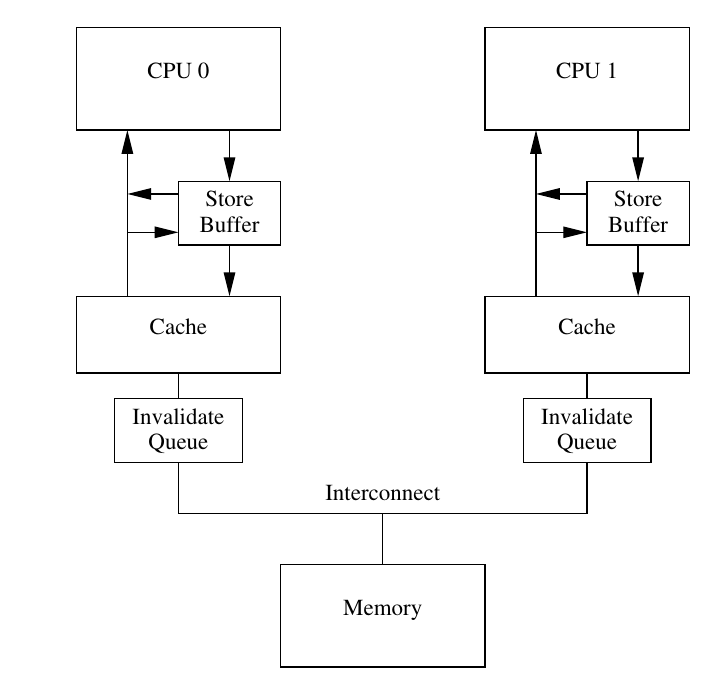
\includegraphics[width=1.\textwidth]{cache-with-wb-iq}
        \end{column}
        \begin{column}{.6\textwidth}
            %			\Large \centering
            解决问题的方法 3: MESI一致性协议
            
            Invalidate  Queue
            
            =================
            
            由于 store buffers的size很小,cpu 执行几个 store 操作就会把
            buffer 填满, 这时候 CPU 必须等待 invalidation ACK 消息,来释
            放缓冲区空间。所以我们在这里引入 Invalidate  Queues。加快invalidate相关的状态转换和cache一致性处理。
            
            
            
            
        \end{column}
    \end{columns}
    
\end{frame}


%----------------------------------------------
\begin{frame}[plain]	
    \frametitle{Introduction -- MESI一致性协议}
    
    
    \begin{columns}
        
        \begin{column}{.4\textwidth}
            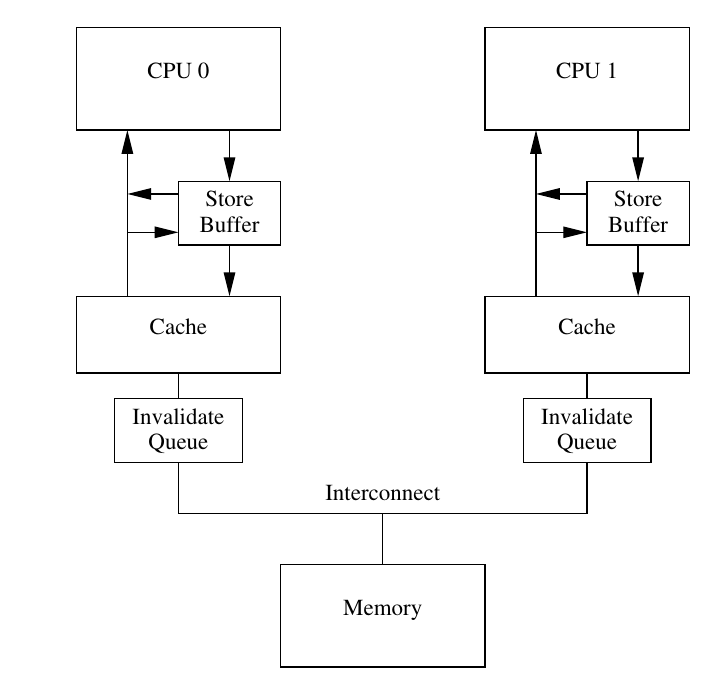
\includegraphics[width=1.\textwidth]{cache-with-wb-iq}
        \end{column}
        \begin{column}{.6\textwidth}
            %			\Large \centering
            解决问题的方法 3: MESI一致性协议
            
            Invalidate  Queue的问题
            
            =================
            
有“Invalidate Queues”的 CPU 会在第一时间将 Invalidate
消息加入队列,并回复 Invalidate Ack,而不用管此时 cache line
是否已被移除。

CPU 在发送回复之前,CPU 需要参考当前的队
列:如果对应的 cache line 已经在队列中,CPU 不能立即发送回
复,而是需要等待这一项被处理后才能回复。

这就导致一个memory misordering问题:当 CPU 排队某个 invalidate 消息后,
在它还没有处理这个消息之前,就再次读取该消息对应的数据
了,该数据此时本应该已经失效的。

        \end{column}
    \end{columns}
    
\end{frame}


%----------------------------------------------
\begin{frame}[plain]	
    \frametitle{Introduction -- MESI一致性协议}
    
    
    \begin{columns}
        
        \begin{column}{.4\textwidth}
            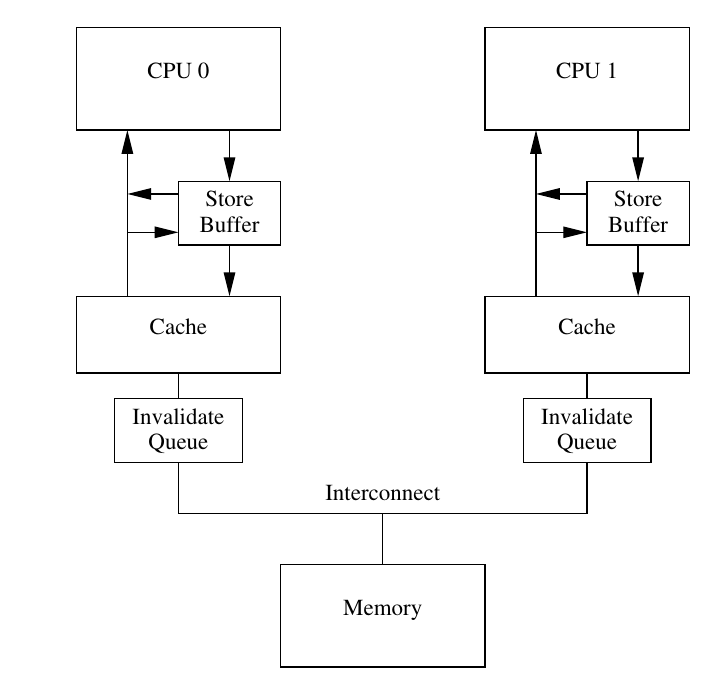
\includegraphics[width=1.\textwidth]{cache-with-wb-iq}
        \end{column}
        \begin{column}{.6\textwidth}
            %			\Large \centering
            解决问题的方法 3: MESI一致性协议
            
            Invalidate  Queue v.s. Memory  Barriers
            
            ==============================
            
            当一个 CPU 执行 memory barrier 指令时,会将失效队列
            中的所有项都做标记,并强制 memory barrier 后续的所有加载都
            要等到标记项被处理后才执行。
            \begin{itemize}
                \item read memory barrier(rmb) 只处理 Invalidate Queues,从而只限制有 rmb 的 CPU
                的 load 操作。
                \item write memory barrier(wmb) 只处理 store buffer,从而只限制有 wmb 的 CPU 的
                store 操作。
                \item 完整的 memory barrier(smp\_mb) 对 Invalidate Queues 和 store buffer 都做标记,
                所以对于 CPU 的 load 和 store 操作都限制。

                
            \end{itemize}
            
        \end{column}
    \end{columns}
    
\end{frame}


%----------------------------------------------
\begin{frame}[plain]	
    \frametitle{Introduction -- MESI一致性协议}
    
    
    \begin{columns}
        
        \begin{column}{.4\textwidth}
            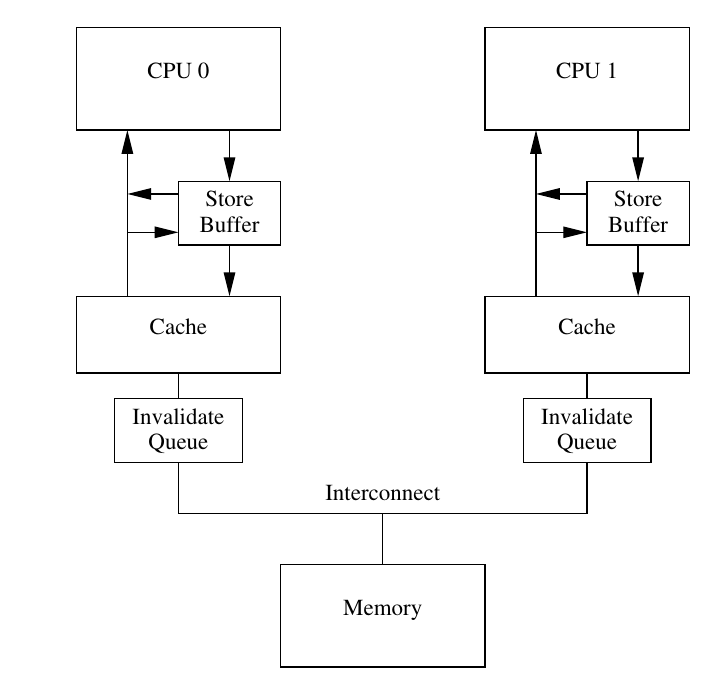
\includegraphics[width=1.\textwidth]{cache-with-wb-iq}
        \end{column}
        \begin{column}{.6\textwidth}
            %			\Large \centering
            在 MC/SMP/NUMA 环境下,我们不能假定:
            

            \begin{itemize}
                \item 一个 CPU 能够按顺序看到另一个 CPU 的访存效果
                \item 与 CPU 相关的硬件会按顺序访存
   
            \end{itemize}
            SMP Read \& Write Memory Barriers 会影响系统中的
            CPU的代码/内存访问顺序,做到代码顺序局部乱序,总体有序。
            
            在内核代码中,如果没有 smp memory barriers 指令,CPU可能会按随意顺序读取 memory,
            这会导致 kernel crash。
            
        \end{column}
    \end{columns}
    \end{frame}
%-------------------------------------------------
\end{document}